\subsection{Application of Random Forest on real data}
\label{sec:real_data}
As previously mentioned, we applied the Random Forest on the Titanic data set \cite{titanicData} in order
to determine the survival of the passengers based on reported attributes like name title or booked cabin.
A major reason for choosing this data set was due to the fact that it consists of many categorical features.
In order to use the data to its fullest extent, we conducted additional feature engineering. 
Without that, many features remain unusable for our methods, 
because they contain missing values or values that are formatted as text.
Further, we split up the data set randomly into five folds via the K-fold method.
Then, the random forest got applied on each of the folds to obtain the classification rates.
Finally, we averaged these results to get a more representative performance evaluation of the Random Forest.
For the implementation of the feature engineering and the classification,
one can consult our code repository \cite{githubApplication}.
The Random Forest managed to achieve a total classification accuracy of 82.71\% on the holdout set.
According to the confusion matrix in figure \ref{fig:confusion_matrix_random_forest}, for passengers that died, 
the accuracy was slightly higher compared to those that survived. This is to be expected,
since deaths outnumber survivals considerably.

\begin{figure}[H]
    \captionsetup{format=plain}
    \makebox[\textwidth]{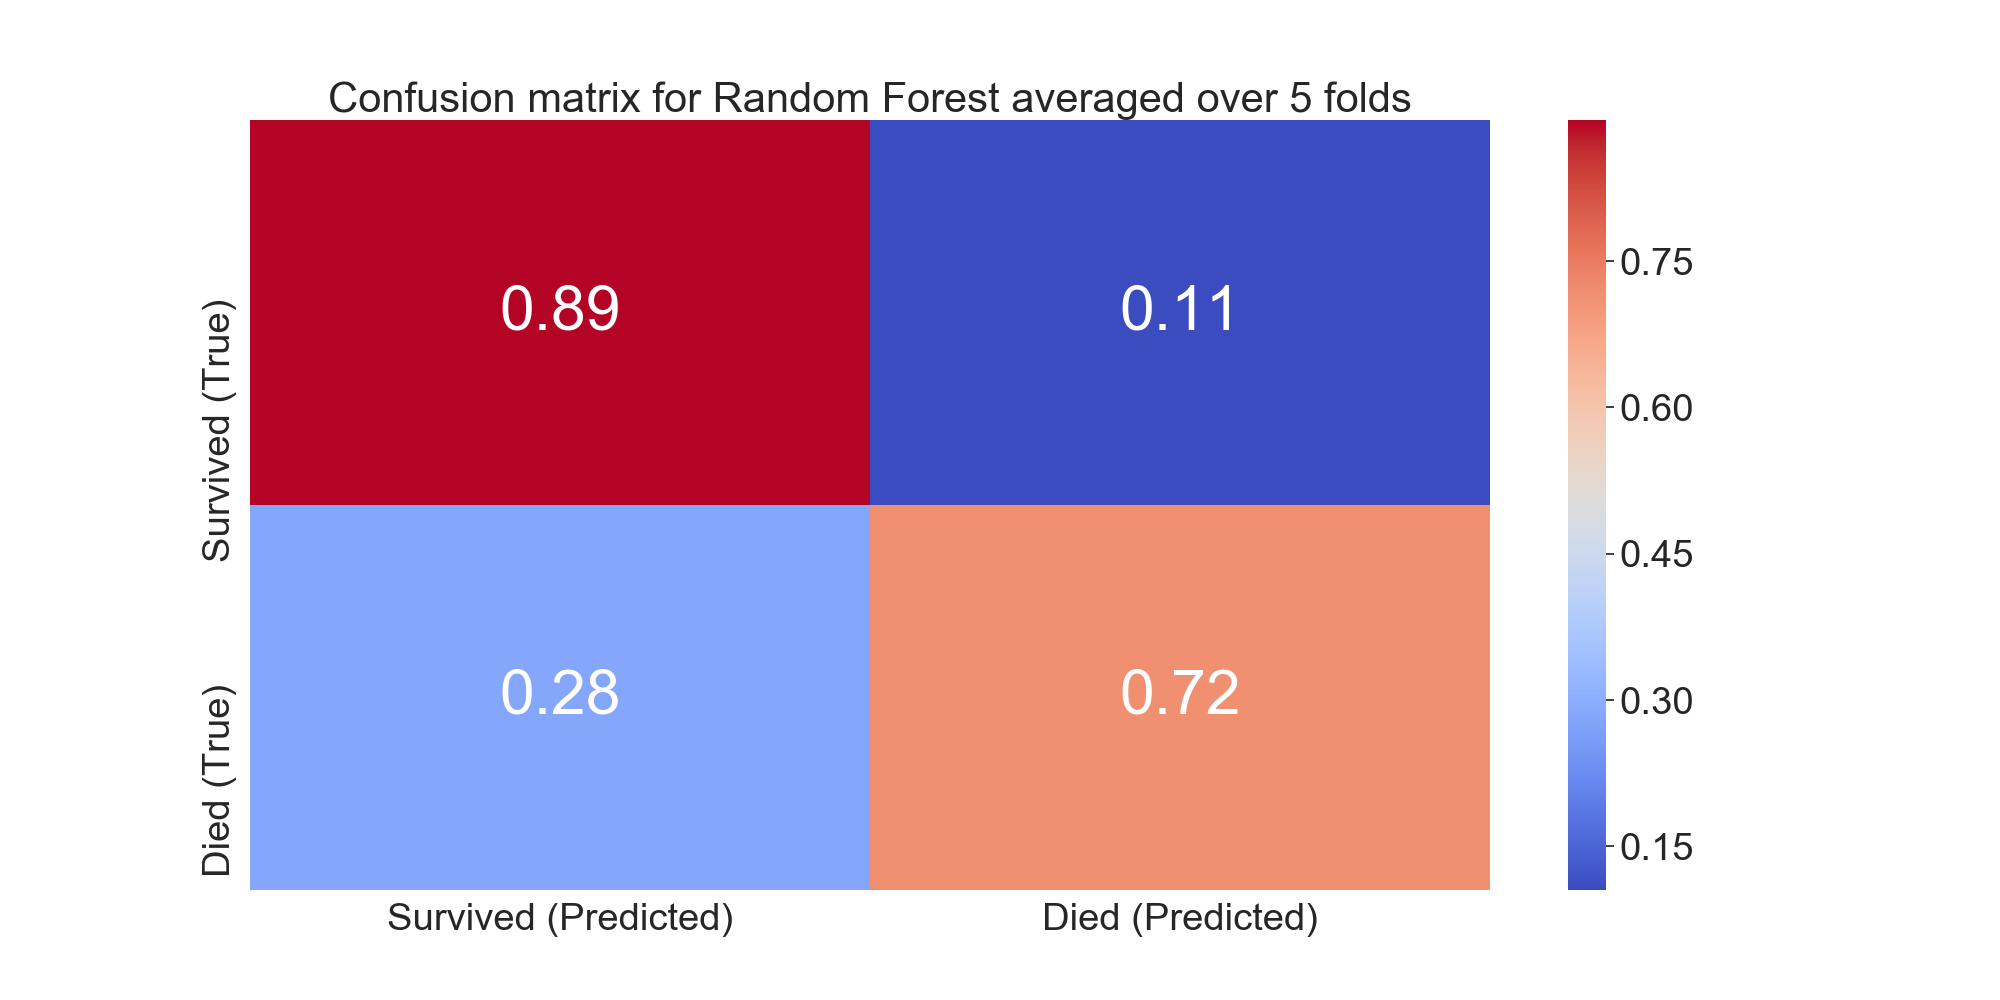
\includegraphics[width=200mm]{confusion_matrix_random_forest.png}}
    \caption
        {This plot illustrates the accuracy of the Random Forest's prediction on the Titanic data set.
        The data set got split into five folds on which the Random Forest got applied. 
        Then, the resulting combination of classification errors got averaged.
        The left axis indicates the true class membership, while the bottom one indicates the predicted one. 
        }
    \label{fig:confusion_matrix_random_forest}
\end{figure}


\section{Comparison to two boosting methods}
Before introducing AdaBoost and Gradient Boosting methods firstly, 
it is essential to understand what boosting is. 
Like bagging, boosting is an approach which can be applied to many machine learning methods for 
classification or regression. Bagging uses bootstrap to create multiple datasets for training the method. 
As a next stage bagging fits a separate Decision Tree to each training dataset, 
and then it combines all Decision Trees in order to create a single predictive model. 
Every Decision Tree is independent to others thanks to using bootstrap to create different training datasets. 
Boosting method works similarly, but in our case Decision Trees are grown sequentially. 
It means that each tree is built using information from previously built trees. 
Boosting method does not involve bootstrap sampling. 
In this method instead of bootstrap each Decision Tree is fit on a modified version of 
the original dataset \cite{James2013}.

\subsection{AdaBoost Classifier}
\label{sec:adaboost}

\subsubsection{An introduction to the AdaBoost method}
Adaptive Boosting (Adaboost) was introduced by \cite{freund1997boosting} and we employ Adaboost as a comparison 
technique against Random Forest. In the Adaboost algorithm, instead of fully-grown trees as in Random Forest, 
we use trees with only one internal node and two leaves also called stumps. We consider those as weak-learners 
compared to trees since its depth and power is limited. Before generating stumps, 
we assign weights to observations in the sample, normally the weight of each observation takes the value 
of $1/N$ as $N$ is the sample size. We generate a stump for each classifier in the data and compare them regarding 
their misclassification rate. After selecting the best classifier, with using its stump's misclassification rate 
we compute its stump's significance. With that significance, we compute new weights for the sample. 
We repeat the algorithm sequentially for the sample with new weights until a stopping criterion is achieved. 
Generally, using the number of classifiers as the number of iteration is a common practice \cite{friedman2001elements}. 
After generating multiple stumps, we can predict an observation's class. 
We get the decision of every stump and form groups accordingly. 
Every outcome class has a group of stumps which predict that class and every stump has its significance. 
After summing significance values of stumps in each group, the prediction is the class with the total highest significance. 
Although stumps are weak-learners, we exploit the error of a weak-learner to generate another weak-learner 
and iterating multiple times provides us with a powerful algorithm.

\subsubsection{Real Data Application of Adaboost}
The application of Adaboost is analogous to that of the Random Forest. 
That means that it got applied on the same five folds from the data set and its results got averaged.
Thus, when we employ Adaboost to predict the survival outcome of the passenger on Titanic, 
we achieve a mean classification rate of 82.94\% accuracy. With utilizing the confusion matrix of Adaboost 
and compare it with Random Forest's, we can see that for the non-survivals the result is almost the same 
but Random Forest is better when it comes to identify survivors.

\begin{figure}[H]
    \captionsetup{format=plain}
    \makebox[\textwidth]{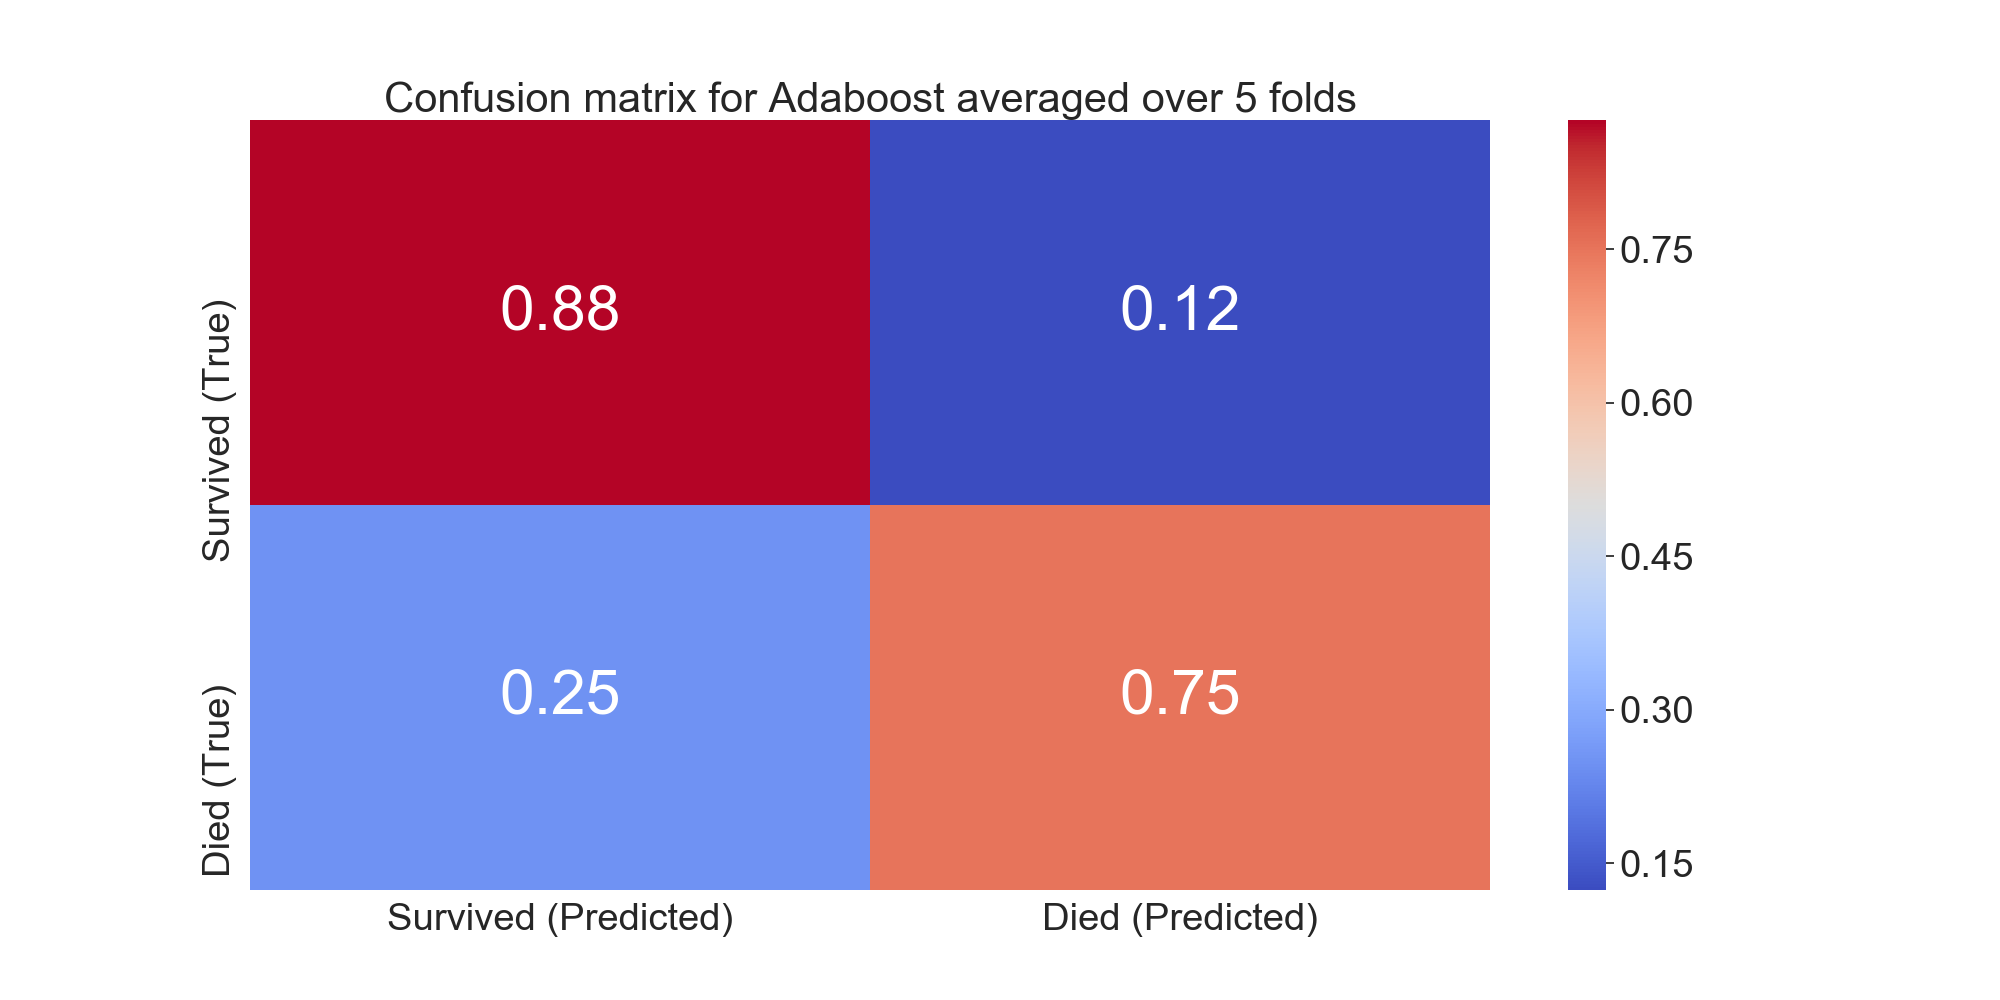
\includegraphics[width=200mm]{confusion_matrix_adaboost.png}}
    \caption
        {This plot illustrates the accuracy of the AdaBoost's prediction on the Titanic data set.
        The data set got split into five folds on which the Random Forest got applied. 
        Then, the resulting combination of classification errors got averaged.
        The left axis indicates the true class membership, while the bottom one indicates the predicted one.
        }
    \label{fig:confusion_matrix_adaboost}
\end{figure}


\subsection{Gradient Boosting Classifier}
\label{sec:gradient_boosting}

\subsubsection{An introduction to the Gradient Boosting method}
In Gradient Boosting the idea is to take weak learning algorithm or hypothesis and make some corrections that will improve the power of this algorithm/hypothesis. In hypothesis boosting, we check every observation on which statistical learning method was trained on, then you leave the observations which were correctly classified. Then method creates new weak learner and test it only on the observations that were poorly classified. Next, the examples that were correctly classified are kept.
The idea described above was used in the AdaBoost algorithm. In this algorithm, many weak learners are created by many Decision Trees that only have a single split. Created instances in the training dataset are weighted in the way that larger weights are assigned to instances which were difficult to classify. To the most difficult training instances weaker learners are added sequentially.
Gradient boosting classifiers are the Adaptive Boosting method, but it is combined with weighted minimization. After weighted minimization, all classifiers and weighted inputs are again calculated. The aim of gradient boosting classifiers is to minimize the loss and it operates in the similar way, as gradient descent in a neural network.

\subsubsection{Real data example}
The application of Gradient Boosting is analogous to that of the other methods. 
That means that it got applied on the same five folds from the data set and its results got averaged.
Thus, when we employ Gradient Boosting to predict the survival outcome of the passenger on Titanic, 
we achieve a mean classification rate of 82.15\% accuracy.

\begin{figure}[H]
    \captionsetup{format=plain}
    \makebox[\textwidth]{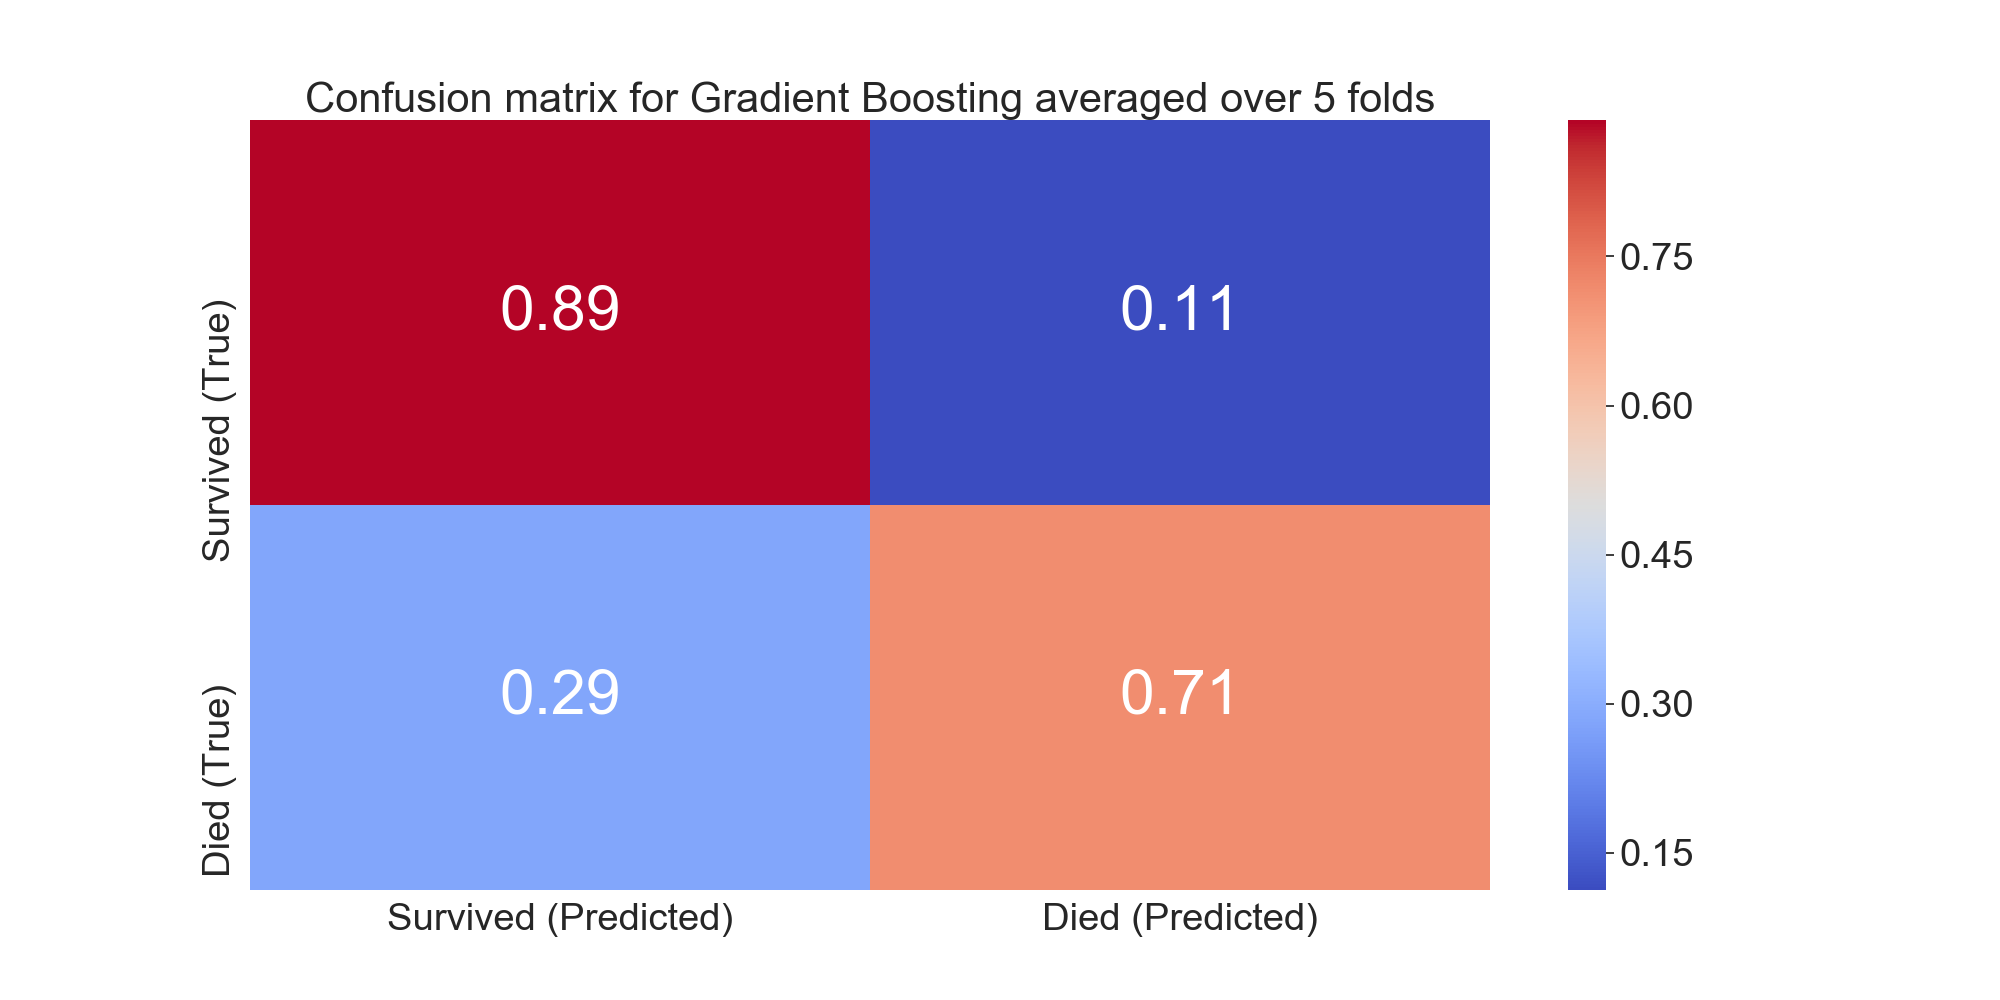
\includegraphics[width=200mm]{confusion_matrix_gradient_boosting.png}}
    \caption{This plot illustrates the accuracy of the Gradient Boosting's prediction on the Titanic data set.
    The data set got split into five folds on which the Random Forest got applied. 
    Then, the resulting combination of classification errors got averaged.
    The left axis indicates the true class membership, while the bottom one indicates the predicted one.}
    \label{fig:confusion_matrix_gradient_boosting}
\end{figure}

